\documentclass[rapport.tex]{subfiles}

\begin{document}
\section{Implementering}
	\subsection{Indledning}
	\subsection{Bruger-interface og applikation}
	I følgende afsnit vil implementeringen af bruger-interfacet og applikationen blive beskrevet. 
	

	\subsubsection{UserInterface}

	\begin{figure}
	\centering
	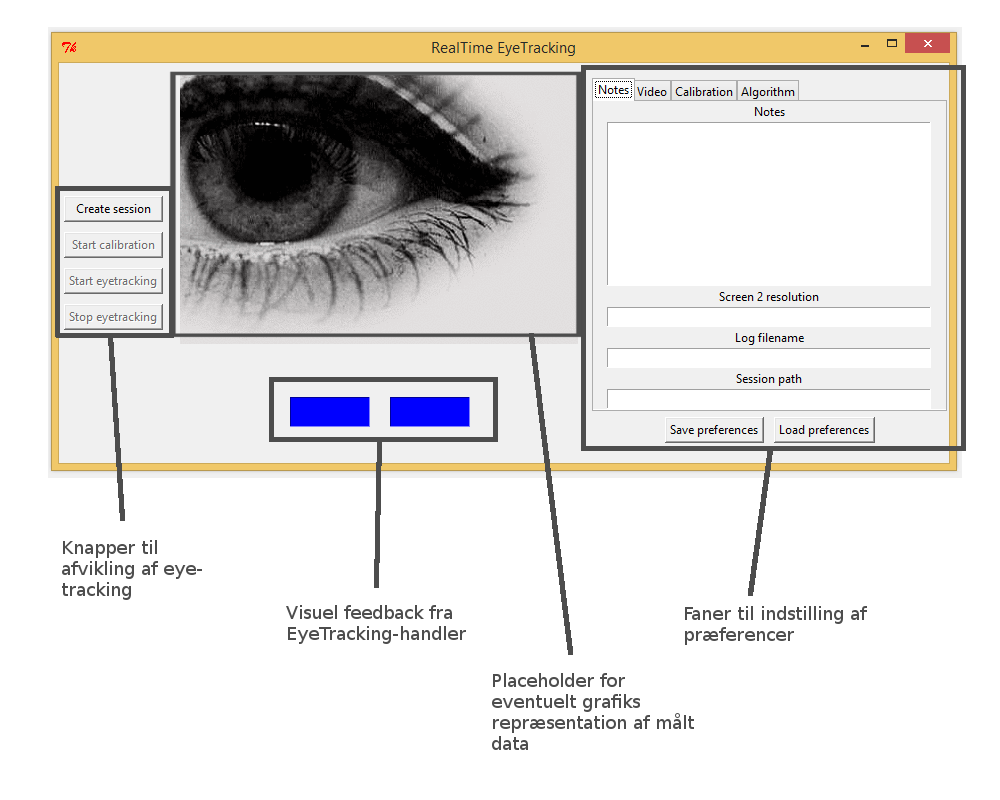
\includegraphics[width=0.9\linewidth]{GUIkommentare}
	\caption[Implementering af GUI]{Implementeringen af det grafiske user-interface med kommentarer}
	\label{fig:GUIkommentare}
	\end{figure}
	
	Tkinter objekter (se afsnit \ref{sec:relBib}) er benyttet til at opbygge det grafisk brugerinterface som givet i design. 
	Hver knap er blevet oprettet med et tilknyttet funktionskald der udfører den ønskede funktion, som givet af de forskellige use cases. 
	Brugeren ser kun Tkinter objekter. 
	Knapperne til venstre i interfacet er sat i rækkefølge efter naturlig opsætning og eksekvering af real-time eye-tracking. Ikke tilgængelige funktioner har deaktiverede knapper således at man ikke kan foretage ulovlige handlinger. \\
	
	De fire faner til højre er til indstilling af præferencer. Herfra kan man tilgå, læse og ændre alle præferencer, samt gemme og indlæse præference-filer.\\
	
	I bunden af bruger-interfacet er to farvede bokse. Disse bokse bruges til at give visuelt feedback bestemt af klassen EyeTrackingHandler. Farven blå indikerer at der ikke kører nogen eye-tracking. Grøn indikerer at eye-tracking kører. Igennem EyeTrackingHandler er det muligt at sætte farven på de to bokse til rød, hvilket kan bruges til at indikere eventuelle fejl. I denne implementering med Starburst-algoritmen er hver boks sat til at repræsentere et øje, således at rød farve indikerer at algoritmen ikke kan finde det tilsvarende øje. 
	Interaktion med andre klasser:
	For hver tilgang til præference-filen bliver der oprettet en ny instans af dataklassen SessionData fra klassen SessionHandler. Ved at aflæse indholdet/værdien af de forskellige Tkiner-objekter og skrive dette data til den instansen af SessionData, der senere bliver skrevet til præference-filen af klassen SessionHandler, vil der altid være konsistens mellem værdierne skrevet i brugerinterfacet, værdierne i præference-filen, og værdierne brugt i eye-tracking-algoritmen. 
	
	Programbibliotekerne tkFileDialog og tkMessageBox giver værktøjer til at kommunikere med brugeren. tkFileDialog håndterer arbejdet med valg af filer, og giver brugeren mulighed for at bevæge sig rundt i mapper på computeren. tkMessageBox bruges til pop-up-vinduer, hvilket benyttes til at tvinge brugeren til at gennemføre valg for at fortsætte, samt til at prompte brugeren om fejl og ulovlige handlinger. 
	
	
	\subsubsection{SessionHandler}
	SessionHandlers opgave er at stille et data-format til rådighed for kommunikation af sessions-indstillinger de forskellige klasser imellem. Klassens vigtigste opgave er derfor at opretholde et korrekt format. Ved oprettelse eller opdatering af præference-fil, kreerer SessionHandler en streng med henholdsvis navn på variabeltype, variable værdi konverteret til streng (hvis variablen er tom, skrives strengen "None"), efterfulgt af et linebreak. Når strengen er oprettet for alle variabler, skrives strengen til en præference-fil med suffiks .pref. \\
	Når en præference-fil indlæses, verificeres den først af SessionHandler ved at lede efter alle variablenavne i den læste fil. Herefter kan hver variabel udtrækkes fra filen. Det er nødvendigt at lave tjek på hver variabel, da konvertering fra python- og numpy-værdi til streng kan medføre komplikationer. 
	
	Instanser af SessionHandler brugt som data-format bliver oftest omtalt som SessionData.\\
	
	Figur \ref{list:sessionfile} er et eksempel på præference-fil med korrekt format (Værdierne variablenames og variablevalues er trunkeret for formateringens skyld). 
\begin{figure}
\caption{Eksempel på præference-fil}
\label{list:sessionfile}
\begin{lstlisting}
SESSIONPATH C:/RealTimeEyeTracking
USINGCAM True
CAMNR None
VIDEOPATH 0
NOTES Dette er en testsession
RESOLUTION 1600x900
CALTYPE Numbers
LOGFILENAME testlog
CALFILENAME testcallog
LOADEDCALDATA None
RECORDVIDEO False
RAWDATAPATH None
VARIABLENAMES['e_center', 'last_eyes', ...
VARIABLEVALUES['[0,0]'$  '[]'$ 'True'$ '20'$ '1500'$ ...
\end{lstlisting}
\end{figure}
		
	\subsubsection{LogHandler}
	For hver eye-tracking måling der igangsættes bliver der oprettet en instans af LogHandler klassen med argumentet SessionData, som er en instans af klassen SessionHandler. LogHandler-klassen består af tre simple funktioner: StartNewTracking, StopTracking og LogData. StartNewTracking er en del af kommunikationsvejen fra UserInterface til EyeTrackingHandler, og har til formål at pege på sig selv, således at EyeTrackingHandler kan kalde LogData i den rette instans af klassen. 
	Ligeledes StartNewTracking er StopTracking en del af kommunikationsvejen, men har kun til formål at sætte klassens variabel Tracking til False. Funktionen LogData bliver kaldt fra EyeTrackingHandler med en streng som argument, og har til formål at skrive denne streng - efterfulgt af et linebreak - til en log-fil peget på af SessionData.  
	
	Figur \ref{list:logfile} er et eksempel på en log-fil med korrekt format (Timestamp, X, Y, Triggerniveau, Fejlmeddelelse). 
\begin{figure}
	\caption{Eksempel på log-fil}
	\label{list:logfile}
	\begin{lstlisting}	
16:28:46.483000, 89, 69, 0, None
16:28:46.662000, 89, 69, 0, None
16:28:46.731000, 90, 70, 0, None
16:28:46.782000, 90, 71, 0, None
16:28:46.951000, 92, 74, 0, None
16:28:47.093000, 89, 68, 0, None
16:28:47.244000, 89, 51, 1, None
16:28:47.322000, 89, 52, 1, None
16:28:47.360000, 91, 52, 1, None
16:28:47.395000, 89, 51, 1, None
16:28:47.598000, 0, 0, 0, Maximum ransac iterations exceeded
16:28:47.651000, 89, 51, 1, None
\end{lstlisting}
\end{figure}	
	
	\subsubsection{CalibrationHandler}
	Vis eksempel på kalibrerings-fil
	
	\subsubsection{EyeTrackingHandler}
	Ved implementering af denne klasse har det været vigtigt at gøre en række overvejelser angående modulariseringen af koden, da det er denne klasse der indirekte står for afviklingen af algoritmen. Funktionen StartVideoCapture bliver kaldt med data-formatet SessionData og en pointer til den relevante instans af LogHandler-klassen. Funktionen opretter en instans af klassen VideoCapture med de korrekte argumenter taget fra SessionData.
	Funktionen StopVideoCapture kalder blot funktionen StopTracking fra klassen VideoCapture, og sætter variablen running til returværdien derfra.\\
	 
	For at sørge for at algoritmen kan afvikles uden forstyrrelser ved opdateringen af det grafiske bruger-interface, indeholder EyeTrackingHandler en EyeTrackingThread-klasse implementeret som en tråd. Når EyeTrackingHandlers funktion StartVideoCapture bliver kaldt, vil en ny process med tråden blive oprettet. Denne tråd vil kalde funktionen updateVideo fra klassen VideoCapture med de valgte argumenter, vente tiden 1/opdateringshastighed, og køre sig selv fra starten så længe at variablen running=True.
	
	Til at modtage data fra algoritmen er de tre funktioner PackWithTimestamp, ReturnError og LastRunInfo. PackWithTimestamp bliver kaldt med argumenterne XY-koordinat og triggerniveau, hvorefter den opretter en streng med den nuværende tid, x-koordinatet, y-koordinatet, triggerniveauet og værdien 'None'. Denne streng sendes derefter som argument til den relevante instans af LogHandler-klassen ved funktionen LogData. ReturnError kan bruges af algoritmen til at returnere fejlmeddelelser. Funktionen modtager fejlmeddelelsen som en streng og opretter en ny streng i samme facon som PackWithTimestamp, blot med koordinaterne (0,0), triggerniveau 0, og fejlmeddelelse. Derefter sendes denne streng også til LogHandler-klassens LogData. LastRunInfo giver algoritmen mulighed for at ændre i de ti frie variabler. Variablerne modtages af algoritmen som argument til funktionen LastRunInfo, der derefter opdatere variablerne i SessionData, således at de bliver benyttet næste gang updateVideo kører. Herved er der fri mulighed for at sende værdier så som fejlmeddelelser, sidste kendte koordinater og så videre tilbage til algoritmen. 
	
	\subsubsection{VideoCapture}
	Indeholder puplic funktion GetCameraInputs, som kan tilgås uden instantiering af klassen. GetCameraInputs detekterer antal kameraer tilsluttet computeren ved at iterere igennem en liste af kamera-inputs givet af operativsystemet. Når et indeks på listen returnere en fejl, returnerer funktionen antal kameraer fundet inden fejlen.\\
	
	De andre funktioner kan først tilgås når klassen er instantieret. Klassen instantieres med et video-input, og mulighed for kalibreringsdataet, samt ti frie variabler. Kalibreringsdataet og de ti frie variabler benyttes ikke til andet end at videresende til ETAlgorithm sammen med gyldig frame. 
	At passe kalibreringsdataet og de frie variabler igennem VideoCapture er ikke optimalt, men spiller ingen rolle i det samlede arbejdslæs. Det kan forestilles at man i stedet ville sende to pointers til hvor disse data ville være lageret. Argumentet for at passe disse data igennem VideoCapture er, at VideoCapture så vil kalde ETAlgorithm's Track() med den fundne frame samt disse data, i stedet for at returnere den fundne frame til EyeTrackingHandler og derefter kalde Track(). VideoCapture håndterer al kommunikation med video-kameraer, og har tilsvarende ansvaret for at terminere forbindelsen med disse når en måling er overstået. 
		
	\subsubsection{Kommunikation imellem applikationens klasser}	
	
	Overordnet kan programmet befinde sig i tre stadier: NotRunning, Calibrating og Running.
	Næsten alle klasser har en variabel der fortæller hvor vidt algoritmen kører eller ej. Herved kan det sikres at systemet ikke forsøger at instantiere klasser, åbne video-inputs, eller overskrive filer der, allerede er i brug.
	
	\subsection{ETAlgorithm}
	Koden i figur \ref{list:emptyalg} er en tom udgave af klassen ETAlgorithm med de nødvendige input-argumenter og funktionskald til EyeTrackingHandler er implementeret:

\begin{figure}
	\caption{Tom udgave af klassen ETAlgorithm}
	\label{list:emptyalg}
\begin{lstlisting}
import numpy as np
import EyeTracking as et

#Her tilfoejes diverse python-biblioteker

def Track(frame, calibration_data, variables):

#Egen kode her 

	et.PackWithTimestamp(screen_point, trigger_value)
	et.LastRunInfo(variables)
	return
\end{lstlisting}
\end{figure}

	
	
	Afsnit \ref{StarburstImpl} beskriver implementering af Starburst-algoritmen i ETAlgorithm.
	\subsection{Starburst-algoritmen}
	\label{StarburstImpl}
	\subsection{Optimering}
	
	\subsubsection{Fremtidige optimeringsmuligheder}
	Python understøtter multitrådning, hvilket giver mulighed for at køre flere instanser af eye-tracking-algoritmen sideløbende. Skriv mere om muligheder for multitrådning, og hvorfor det kan virke.
	\subsection{Diskussion}
		
\end{document}